% ==================
% Landon Buell
% Keesee
% PHYS 708.01
% 6 October 2019
% ==================

\documentclass[12pt,letterpaper]{article}
\usepackage{graphicx}
\usepackage{multicol}
\usepackage[left=2.5cm,right=2.5cm,top=2.5cm]{geometry}
\usepackage{enumitem}
\usepackage{fancyhdr}
\setitemize{noitemsep,topsep=0pt,parsep=0pt,partopsep=0pt}

\pagestyle{fancy}
\fancyhf{}
\rhead{\thepage}
\lhead{Modeling a Simple Optical System}

% ==================

\begin{document}

% ======================================================

\title{
\begin{Huge}
Modeling a Simple Optical System\\
\end{Huge}
\vspace*{5mm}
\Large Numerically Modeling a One - Dimensional Optical System in Python 3}
\author{Landon Buell}
\date{PHYS 708.01 - Fall 2019}
\maketitle


% ======================================================

\section{Abstract}
\paragraph*{}A classical optics, a system of thin lenses can be solved analytically by use of several pertinent equations and geometric principles. As these systems become increasingly complex, the volume of math and geometry require increases drastically, meaning that a system becomes more and more prone to calculation error. In order to combat this, I have developed a a program that will algorithmically evaluate the components of an optical system. Component $m$ will take object/image $m-1$ and use the \textit{thin lens law} to produce object/image $m$. The in a system with $N$ components, the image $m = N$ will be the final image as produced by the entire system.

% ======================================================

\section{Introduction}
\paragraph*{}This project will see the creation of a python 3 program that can efficiently and accurately model a simple, ideal, one - dimensional optical system. All components in the system will be assumed to adhere to all classical models and equations. Due to complexity, all possible systems may not be physically realistic. The legitimacy of each simulation is bound only by mathematical rules.
\paragraph*{}The program will revolve around a few basic optical principles as learned from class (PHYS 708 - Optics) as well as from various other references. For all computations, light will be assumed to be an perfectly idealized geometric ray. The exact wavelength of the ray will not change the index of refraction of the object as well.

\pagebreak
% ======================================================

\section{General Methodology}
\paragraph*{}The functionality of this project will rely on object-oriented programming. Additionally, all mathematics are based on classical optical laws. The needed ones are: \\

The \textbf{Lens Maker's Equation}
\begin{equation}
\label{lens maker}
\frac{1}{f} = (n_l - 1)\bigg(\frac{1}{R_1} - \frac{1}{R_2}\bigg)
\end{equation}

\textbf{Gaussian Lens Formula}
\begin{equation}
\label{gauss}
\frac{1}{s_o} + \frac{1}{s_i} = \frac{1}{f}
\end{equation}

\textbf{Transverse Magnification factor}
\begin{equation}
\label{mag fact}
M_T = -\frac{s_i}{s_o}
\end{equation}

\paragraph*{} In all cases, the previous parameters are defined:
\begin{itemize}
\item[•]$f$ - lens focal length from center of lens (cm)
\item[•]$n_l$ - index of refraction of lens
\item[•]$R_1$ - Radius of curvature of left side of lens (cm)
\item[•]$R_2$ - Radius of curvature of right side of lens (cm)
\item[•]$s_o$ - object distance from center of lens (cm)
\item[•]$s_i$ - image distance from center of lens (cm)
\item[•]$M_T$ - Transverse Magnification factor
\end{itemize}

% ==================

\subsection{Optical Components Object}
\paragraph*{}The computational part of this program will involve the construction of a \textit{class} object that will contain all attributes that are relevant to modeling the system.
\paragraph*{}The main class object used will be the \textit{Thin Lens} object. Each lens in the system will be an additional instance of this class. It will be defined:
\begin{verbatim}
class Thin_Lens ():
    """
    Creates Thin Lens Class Object
    --------------------------------
    name (str) : Name to indentify object
    x (float) : Position on x-axis where center of lens sits
    ref_idx (float) : index of refraction of thin lens
    R1 (float) : radius of curvature 1 of lens
    R2 (float) : radius of curvature 2 of lens
    --------------------------------
    """
\end{verbatim}
Attributes: \textit{component name}, \textit{component position},\textit{index of refraction}, \textit{Radius of Curvature 1}, \textit{Radius of Curvature 2}, \textit{Component Focal length}, \textit{lense component type}.
\subsubsection*{Initialization}
\paragraph*{}As per convention, the optical component object will begin with an \textbf{\_\_init\_\_()} method to set all object attributes. In python, this method takes the form:
\begin{verbatim}
def __init__(self,name,x,ref_idx,R1,R2):
    """ Initiaialize Thin Lens Class Object """
    self.name = name            # name of object
    self.x = x                  # horizontal position
    self.n = ref_idx            # refraction idx
    self.R1 = R1                # rad of curve 1
    self.R2 = R2                # rad of curve 2
    self.f = self.focus()       # focal length
    self.type = self.lens_type()# lens type
\end{verbatim}
\paragraph*{}The method \textit{self.focus()} comutes the focal distance of the lens class instance based on the \textit{Lens Maker's Equation}, Equation (\ref{lens maker}). The \textit{self.lens\_type()} method determines the type of thin lense based on the two radii of curvature, as defined below:

\subsubsection*{Other Methods}

\paragraph*{}The \textit{Thin\_Lens()} class must have method that allows for the computation of the image distance as measured from the center of the thin lens.  This will be computed as per the \textit{Gaussian Lens Formula}, Equation (\ref{gauss}). It is defined:
\begin{verbatim}
def image_distance(self,obj):
    """ Compute image distance from lens instance """
    d = obj.x - self.x              # distance between obj & lens
    si = (1/self.f - 1/d)**-1       # image distance
    return si                       # return image distance 
\end{verbatim}
\paragraph*{}Using this image distance $s_i$, and the horizontal position of the center of the lens from the origin of the coordinate system. Note that this method uses the parameter \textit{obj} which is the class object that represents the physical image or object.

\paragraph*{}The textit{Thin\_Lens()} class also has a method for determining it's lens type. As defined by standard optical lens conventions, The method uses the radii of curvature and a series of if statements. it is defined:
\begin{verbatim}
def lens_type(self):
    """ Determine lens type based on radii of curvature """
    if (self.R1 > 0) and (self.R2 < 0):
        return 'Biconvex'           # biconvex lens
    if (self.R1 > 1e6) and (self.R2 < 0):
        return 'Planar - Convex'    # planar convex lens
    if (self.R1 > 0) and (self.R2 > 0):
        return 'Meniscus - Convex'  # meniscus convex len
    if (self.R1 < 0) and (self.R2 > 0):
        return 'Biconcave'          # bicondave lens
    if (self.R1 > 1e6) and (self.R2 > 0):
        return 'Planar - Concave'   # planar concave lens
    if (self.R1 > 0) and (self.R2 > 0):
        return 'Meniscus Concave'   # meniscus concave lens
\end{verbatim}
\paragraph*{}The simplification has been made where if the radius of curvature of a lens is greater than $10^{6}$ units, it is treated as if to have an 'infinite' radius of curvature - i.e. it is a flat surface. This was made to handle large values, and potentially infinite ones.

% ==================

\subsection{Object \& Image Object}
\paragraph*{}The image produced from each lens will serve as the object for the next one. In this case, objects and images in the system all have the same properties. This can be modeled by creating a \textit{Object/Image} class object. Each successive image/object produced by the system, becomes a new instance of the the class. It is defined:
\begin{verbatim}
class Object_or_Image ():
    """
    Creates Object to image Class Object 
    --------------------------------
    name (str) : Name to identify object
    x (float) : Position on x-axis where center of lens sits
    height (float) : height of object/image
    --------------------------------
    """
\end{verbatim}
Attributes: \textit{image/object name}, \textit{image/object position},  \textit{image/object height}, \textit{image/object number}

\subsubsection*{Initialization}
\paragraph*{}The \textbf{\_\_init\_\_()} method of the class takes the form:	
\begin{verbatim}
def __init__(self,name,x,height,n):
    """ Initialize Object\Image Class Object """
    self.name = name                # name of object
    self.x = x                      # position of object/image
    self.h = height                 # height of object/image
    self.num = n                    # object number
    self.type = self.image_type()   #  type of image
\end{verbatim}
\paragraph*{}Here, all arguments for the class are procedurally generated by the program. Additionally, the type of the image is determined by the method \textit{image\_type()} based on standard classical optics parameters.

\subsubsection*{Other Methods}
\paragraph*{}The \textit{Object\_Image} class also contains a method to determine the \textit{type} of image produced by the system.

% ==================

\subsection{Visualization}
\paragraph*{}Once the system has been tracked computationally, a visualization is produced. This visualization is done in Python's \textit{matplotlib.pyplot} module and contains the position of all optical components, position of respective focii and each successive image as produced by the system. All components are labeled and visualized to scale. The plot will be displayed when the system is finished with all computations. Note that radii of curvature of each lens are not considered in visualization.
\paragraph*{}In addition to the plot, the details for each component and object or image will also be printed out concisely for the ease of human reading. Again, this will happen at the end of the full computation cycle.

% ==================

\subsection{General Procedure}
\paragraph*{}In general, an optical system will contain $M$ optical elements (lenses) and one object to image. The single image object will be stored in a \textit{numpy array}, and all $M$ of the lens objects will be stored in a separate array.
\paragraph*{}The program then iterates through the \textit{lenses} array, using the $m^{th}$ lens object and the $m^{th}$ object to produce the location of the $m+1^{th}$ object. Once the image location and properties are determined, it becomes an instance of the \textit{Object\_Image} class, and gets added to the corresponding array. In the next iteration, it is treated as the new obeject to produce an image of. 
\paragraph*{}This continues until there are $M+1$ objects in the system, i.e. all lenses have successfully used equation (\ref{gauss}) to produce an image from the previous object. The final object, $M+1$, is the final image as viewed by an observer of the entire system.

% ======================================================
\pagebreak

\section{Example System \#1}
\paragraph*{}The first test of the program will be a simple system, containing two lenses. The program prints out the details of each lens:
\begin{verbatim}
================================
Component Number: 1
        Name: Lens 1
        Component type: Biconvex lens
        X-Axis Postion: 100
        1st Curvature radius: 20
        2nd Curvature radius: -20
        Focal length: 20.0

================================
Component Number: 2
        Name: Lens 2
        Component type: Biconvex lens
        X-Axis Postion: 130
        1st Curvature radius: 20
        2nd Curvature radius: -20
        Focal length: 20.0
\end{verbatim}
\paragraph*{}And finally, the visualiztion of the system:
\begin{center}
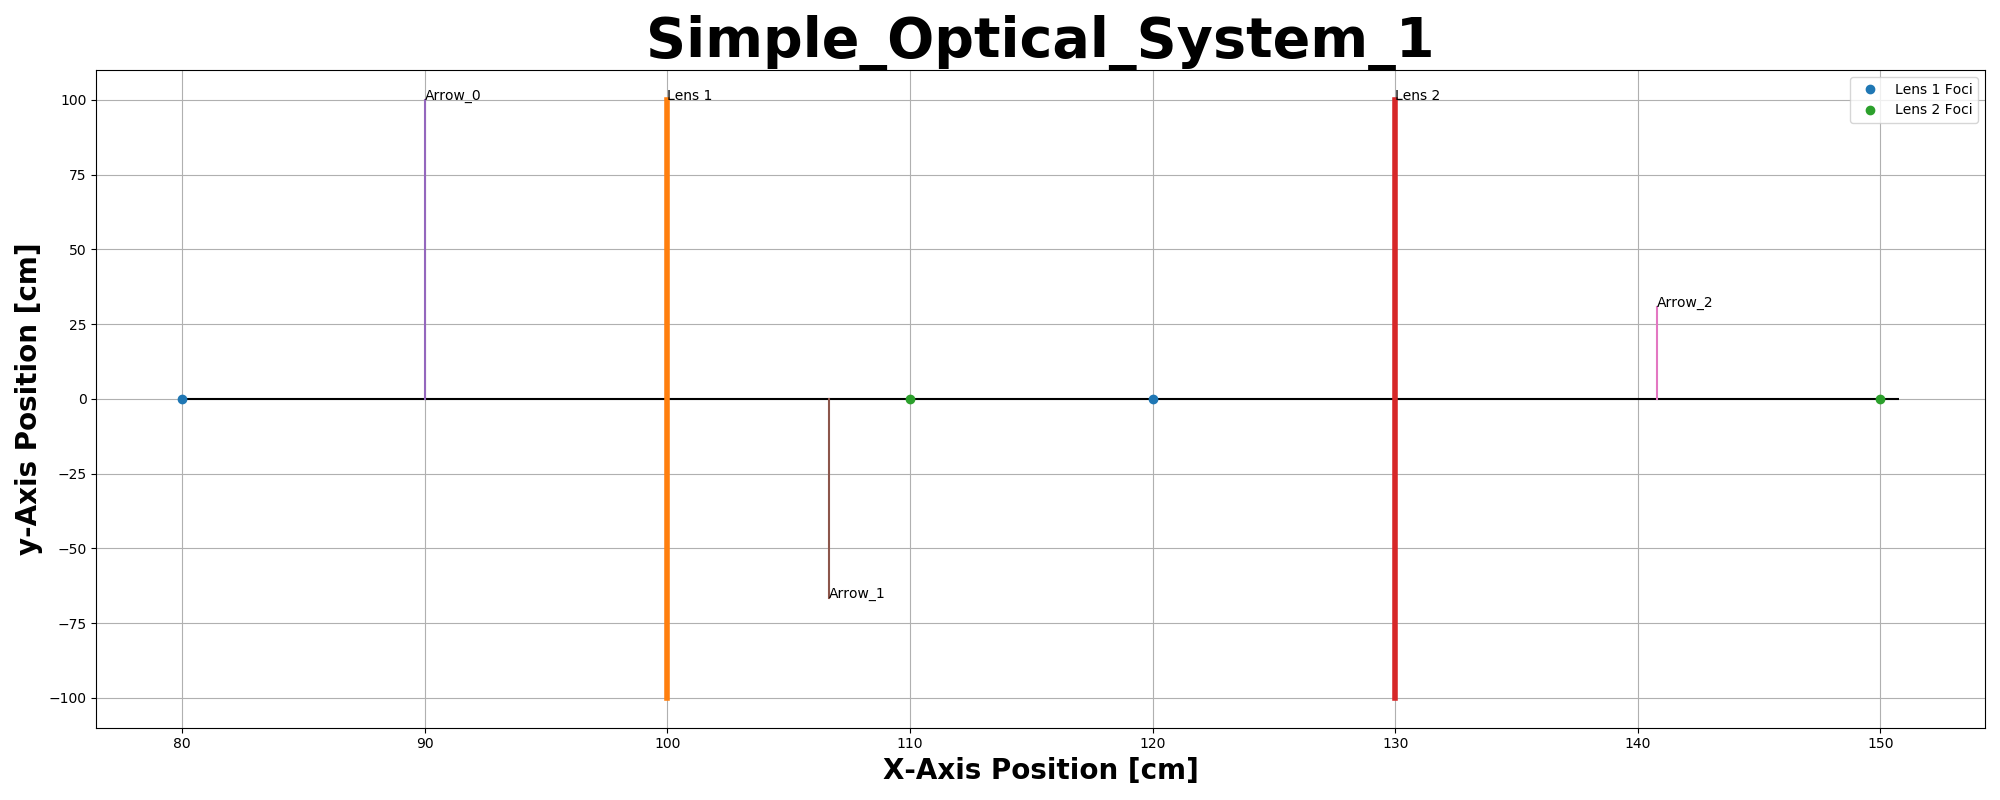
\includegraphics[scale=0.34]{Simple_Optical_System_1}
\end{center}
The legitimacy of the computation can be confirmed by hand or with another program if desired.

% ======================================================

\section{Example System \#2}
\paragraph*{}To test the potential of the program more, we can try to model a far more complex system. We will create an array of 4 lenses, and attempt to image an object through all of them. For the sake of space, I can write the lens parameters as they are hard-coded in:
\begin{verbatim}
lenses = np.array([ OC.Thin_Lens('Lens 1',50.,1.5,+20,-20),
                    OC.Thin_Lens('Lens 2',100,1.2,-40,+40),
                    OC.Thin_Lens('Lens 3',160,2.0,+10,-20),                     
                    OC.Thin_Lens('Lens 4',220,1.5,+20,-20)]) 
\end{verbatim}
The attribute for each parameter is found in the definitions above.
\paragraph*{}At the end of the computations, we print out the attributes for the first and last image:
\begin{verbatim}
================================
Object Number:  0
        Name: Arrow_0
        Image type: None
        X-Axis Postion: 0
        Image Height: 100

================================
Object Number:  4
        Name: Arrow_4
        Image type: None
        X-Axis Postion: 234.82758620689654
        Image Height: 6.896551724137939
\end{verbatim}
\paragraph*{}And Finally, the visualization:
\begin{center}
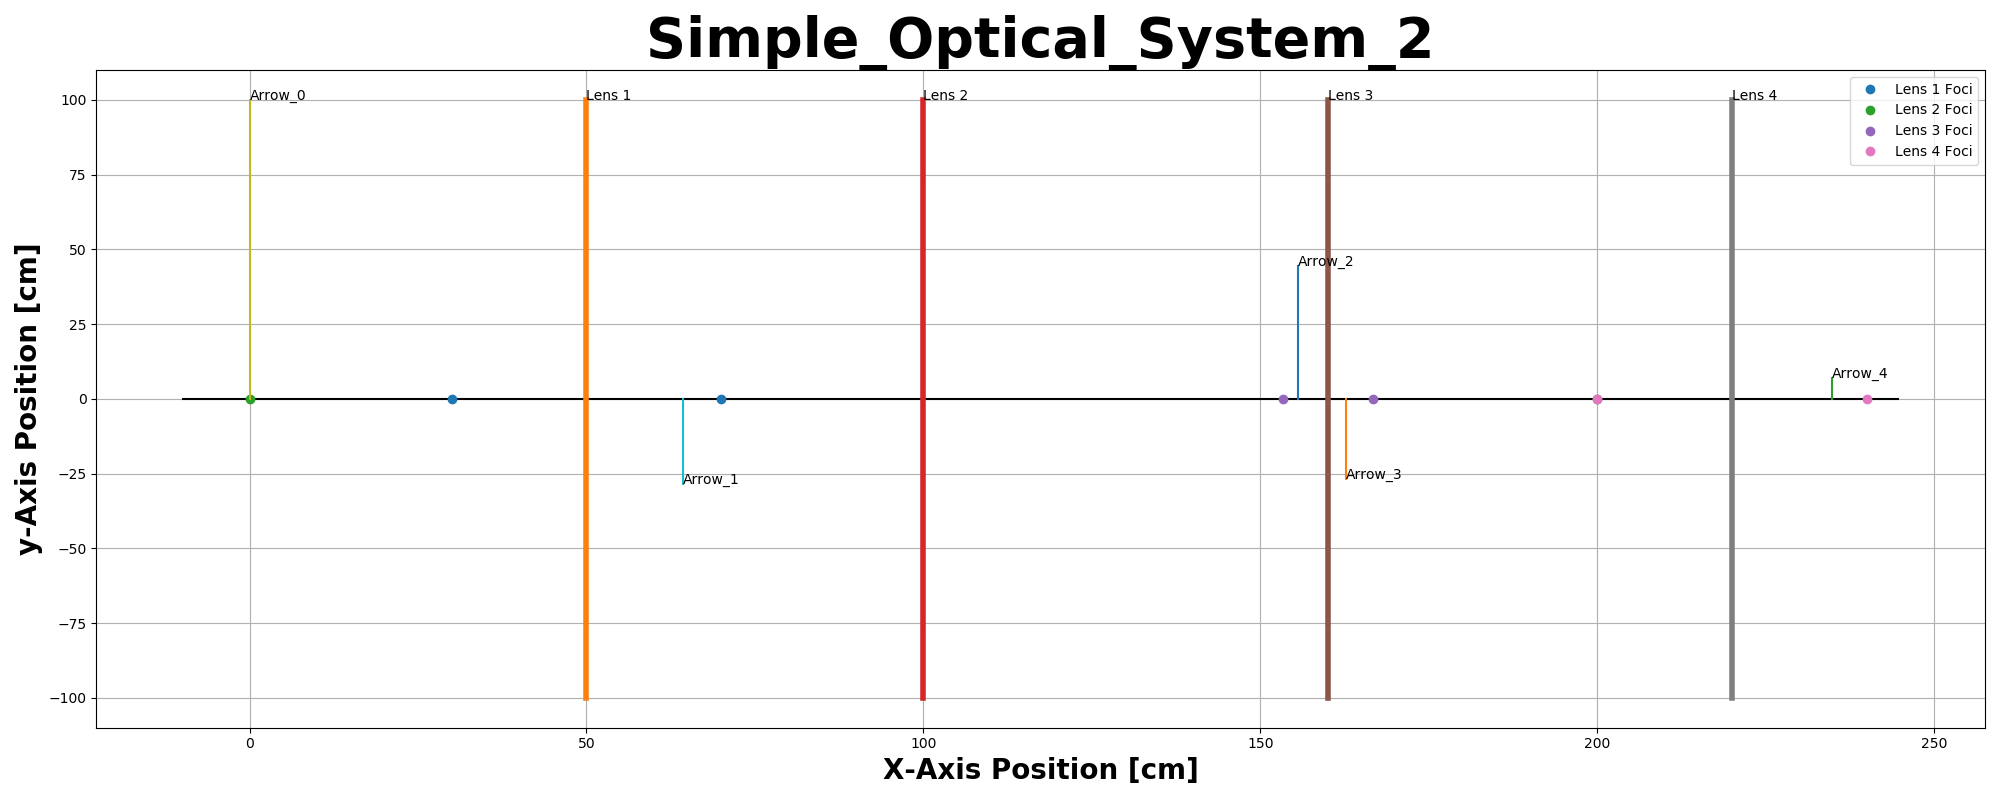
\includegraphics[scale=0.34]{Simple_Optical_System_2}
\end{center}
% ======================================================

\section{Additional Notes}
\begin{itemize}
\item[•]\textbf{Realistic Systems}\\
Due to the lack of detailed error handling, is it possible to attempt to model physically unrealistic systems. These may included (but not limited to): over lapping lenses, infinite or undefined values, etc.
\item[•]\textbf{One Dimensional}\\
The optical system modeled is strictly one dimensional, and all components move left to right. It is also implied at all lenses in the array are ordered by position - i.e. the system does not take in considerations the physical ordering of components, only as listed in the array.
\item[•]\textbf{Python Modules}\\
Required Python Modules: Numpy, Scipy, Matplotlib
\end{itemize}

% ======================================================

\section{Conclusion}
\paragraph*{}With Python, I have created a program to numerically model a simple one dimensional optical system composed of a single object to image and a collection of simple thin lenses. By using object-oriented programming, and the laws of classical optics, the system can iterate through the components to produce a position and height for a final image.

% ======================================================

\section{References}
\begin{itemize}
\item[•]“Geometrical Optics.” Optics, by Eugene Hecht, 5th ed., Pearson, 2017, pp. 151–246.
\end{itemize}
% ======================================================

\end{document}